% Options for packages loaded elsewhere
% Options for packages loaded elsewhere
\PassOptionsToPackage{unicode}{hyperref}
\PassOptionsToPackage{hyphens}{url}
\PassOptionsToPackage{dvipsnames,svgnames,x11names}{xcolor}
%
\documentclass[
  letterpaper,
  DIV=11,
  numbers=noendperiod]{scrartcl}
\usepackage{xcolor}
\usepackage[lmargin=15mm,rmargin=15mm,tmargin=30mm,bmargin=30mm]{geometry}
\usepackage{amsmath,amssymb}
\setcounter{secnumdepth}{-\maxdimen} % remove section numbering
\usepackage{iftex}
\ifPDFTeX
  \usepackage[T1]{fontenc}
  \usepackage[utf8]{inputenc}
  \usepackage{textcomp} % provide euro and other symbols
\else % if luatex or xetex
  \usepackage{unicode-math} % this also loads fontspec
  \defaultfontfeatures{Scale=MatchLowercase}
  \defaultfontfeatures[\rmfamily]{Ligatures=TeX,Scale=1}
\fi
\usepackage{lmodern}
\ifPDFTeX\else
  % xetex/luatex font selection
\fi
% Use upquote if available, for straight quotes in verbatim environments
\IfFileExists{upquote.sty}{\usepackage{upquote}}{}
\IfFileExists{microtype.sty}{% use microtype if available
  \usepackage[]{microtype}
  \UseMicrotypeSet[protrusion]{basicmath} % disable protrusion for tt fonts
}{}
\makeatletter
\@ifundefined{KOMAClassName}{% if non-KOMA class
  \IfFileExists{parskip.sty}{%
    \usepackage{parskip}
  }{% else
    \setlength{\parindent}{0pt}
    \setlength{\parskip}{6pt plus 2pt minus 1pt}}
}{% if KOMA class
  \KOMAoptions{parskip=half}}
\makeatother
% Make \paragraph and \subparagraph free-standing
\makeatletter
\ifx\paragraph\undefined\else
  \let\oldparagraph\paragraph
  \renewcommand{\paragraph}{
    \@ifstar
      \xxxParagraphStar
      \xxxParagraphNoStar
  }
  \newcommand{\xxxParagraphStar}[1]{\oldparagraph*{#1}\mbox{}}
  \newcommand{\xxxParagraphNoStar}[1]{\oldparagraph{#1}\mbox{}}
\fi
\ifx\subparagraph\undefined\else
  \let\oldsubparagraph\subparagraph
  \renewcommand{\subparagraph}{
    \@ifstar
      \xxxSubParagraphStar
      \xxxSubParagraphNoStar
  }
  \newcommand{\xxxSubParagraphStar}[1]{\oldsubparagraph*{#1}\mbox{}}
  \newcommand{\xxxSubParagraphNoStar}[1]{\oldsubparagraph{#1}\mbox{}}
\fi
\makeatother


\usepackage{longtable,booktabs,array}
\usepackage{calc} % for calculating minipage widths
% Correct order of tables after \paragraph or \subparagraph
\usepackage{etoolbox}
\makeatletter
\patchcmd\longtable{\par}{\if@noskipsec\mbox{}\fi\par}{}{}
\makeatother
% Allow footnotes in longtable head/foot
\IfFileExists{footnotehyper.sty}{\usepackage{footnotehyper}}{\usepackage{footnote}}
\makesavenoteenv{longtable}
\usepackage{graphicx}
\makeatletter
\newsavebox\pandoc@box
\newcommand*\pandocbounded[1]{% scales image to fit in text height/width
  \sbox\pandoc@box{#1}%
  \Gscale@div\@tempa{\textheight}{\dimexpr\ht\pandoc@box+\dp\pandoc@box\relax}%
  \Gscale@div\@tempb{\linewidth}{\wd\pandoc@box}%
  \ifdim\@tempb\p@<\@tempa\p@\let\@tempa\@tempb\fi% select the smaller of both
  \ifdim\@tempa\p@<\p@\scalebox{\@tempa}{\usebox\pandoc@box}%
  \else\usebox{\pandoc@box}%
  \fi%
}
% Set default figure placement to htbp
\def\fps@figure{htbp}
\makeatother





\setlength{\emergencystretch}{3em} % prevent overfull lines

\providecommand{\tightlist}{%
  \setlength{\itemsep}{0pt}\setlength{\parskip}{0pt}}



 


\usepackage{fvextra}
\DefineVerbatimEnvironment{Highlighting}{Verbatim}{breaklines,commandchars=\\\{\}}
\KOMAoption{captions}{tableheading}
\makeatletter
\@ifpackageloaded{tcolorbox}{}{\usepackage[skins,breakable]{tcolorbox}}
\@ifpackageloaded{fontawesome5}{}{\usepackage{fontawesome5}}
\definecolor{quarto-callout-color}{HTML}{909090}
\definecolor{quarto-callout-note-color}{HTML}{0758E5}
\definecolor{quarto-callout-important-color}{HTML}{CC1914}
\definecolor{quarto-callout-warning-color}{HTML}{EB9113}
\definecolor{quarto-callout-tip-color}{HTML}{00A047}
\definecolor{quarto-callout-caution-color}{HTML}{FC5300}
\definecolor{quarto-callout-color-frame}{HTML}{acacac}
\definecolor{quarto-callout-note-color-frame}{HTML}{4582ec}
\definecolor{quarto-callout-important-color-frame}{HTML}{d9534f}
\definecolor{quarto-callout-warning-color-frame}{HTML}{f0ad4e}
\definecolor{quarto-callout-tip-color-frame}{HTML}{02b875}
\definecolor{quarto-callout-caution-color-frame}{HTML}{fd7e14}
\makeatother
\makeatletter
\@ifpackageloaded{caption}{}{\usepackage{caption}}
\AtBeginDocument{%
\ifdefined\contentsname
  \renewcommand*\contentsname{Table of contents}
\else
  \newcommand\contentsname{Table of contents}
\fi
\ifdefined\listfigurename
  \renewcommand*\listfigurename{List of Figures}
\else
  \newcommand\listfigurename{List of Figures}
\fi
\ifdefined\listtablename
  \renewcommand*\listtablename{List of Tables}
\else
  \newcommand\listtablename{List of Tables}
\fi
\ifdefined\figurename
  \renewcommand*\figurename{Figure}
\else
  \newcommand\figurename{Figure}
\fi
\ifdefined\tablename
  \renewcommand*\tablename{Table}
\else
  \newcommand\tablename{Table}
\fi
}
\@ifpackageloaded{float}{}{\usepackage{float}}
\floatstyle{ruled}
\@ifundefined{c@chapter}{\newfloat{codelisting}{h}{lop}}{\newfloat{codelisting}{h}{lop}[chapter]}
\floatname{codelisting}{Listing}
\newcommand*\listoflistings{\listof{codelisting}{List of Listings}}
\makeatother
\makeatletter
\makeatother
\makeatletter
\@ifpackageloaded{caption}{}{\usepackage{caption}}
\@ifpackageloaded{subcaption}{}{\usepackage{subcaption}}
\makeatother
\usepackage{bookmark}
\IfFileExists{xurl.sty}{\usepackage{xurl}}{} % add URL line breaks if available
\urlstyle{same}
\hypersetup{
  pdftitle={Homework 6: The Bootstrap and Missing Data},
  pdfauthor={Avinash Aravind, aa2476},
  colorlinks=true,
  linkcolor={blue},
  filecolor={Maroon},
  citecolor={Blue},
  urlcolor={Blue},
  pdfcreator={LaTeX via pandoc}}


\title{Homework 6: The Bootstrap and Missing Data}
\usepackage{etoolbox}
\makeatletter
\providecommand{\subtitle}[1]{% add subtitle to \maketitle
  \apptocmd{\@title}{\par {\large #1 \par}}{}{}
}
\makeatother
\subtitle{BEE 4850/5850}
\author{Avinash Aravind, aa2476}
\date{2026-05-01}
\begin{document}
\maketitle

\RecustomVerbatimEnvironment{verbatim}{Verbatim}{
showspaces = false,
showtabs = false,
breaksymbolleft={},
breaklines
% Note: setting commandchars=\\\{\} here will cause an error
}

\renewcommand*\contentsname{Contents}
{
\hypersetup{linkcolor=}
\setcounter{tocdepth}{3}
\tableofcontents
}

\begin{tcolorbox}[enhanced jigsaw, leftrule=.75mm, colframe=quarto-callout-note-color-frame, colback=white, opacityback=0, bottomrule=.15mm, rightrule=.15mm, colbacktitle=quarto-callout-note-color!10!white, arc=.35mm, bottomtitle=1mm, left=2mm, title=\textcolor{quarto-callout-note-color}{\faInfo}\hspace{0.5em}{Note}, coltitle=black, breakable, toptitle=1mm, titlerule=0mm, toprule=.15mm, opacitybacktitle=0.6]

All of the code used in this homework is accessible in the hw06.ipynb
file in my GitHub repository.

\end{tcolorbox}

\newpage

\section{Problem 1: Salamanders \& the Parametric
Bootstrap}\label{problem-1-salamanders-the-parametric-bootstrap}

\subsubsection{1.1}\label{section}

\begin{figure}[h]

\centering{

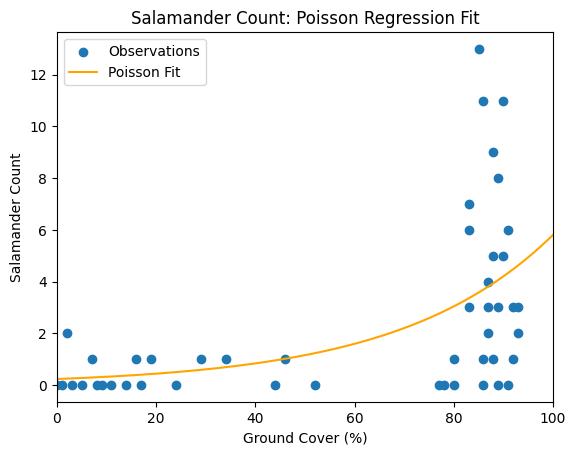
\includegraphics[width=5in,height=\textheight,keepaspectratio]{./images/fig1.png}

}

\caption{\label{fig-1}Scatterplot of Salamander Count vs.~Ground Cover,
with Poisson Regression fit shown in orange.}

\end{figure}%

The intercept from the Poisson Regression fit is -1.478, and the
coefficient from the fit is 0.032.

\newpage

\subsubsection{1.2}\label{section-1}

\begin{figure}[H]

\begin{minipage}{0.50\linewidth}

\centering{

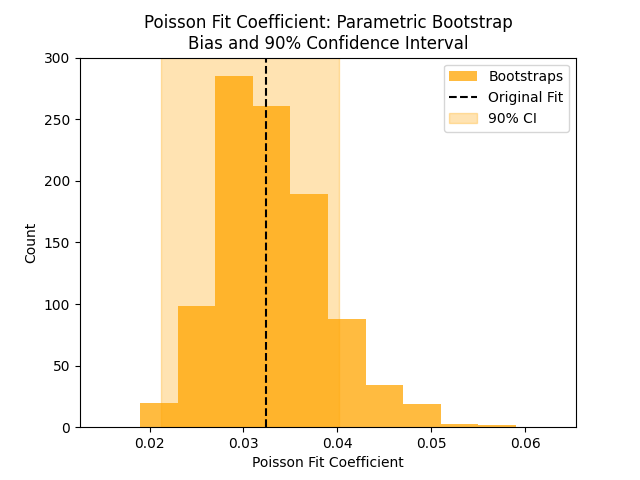
\includegraphics[width=4in,height=\textheight,keepaspectratio]{./images/fig2.png}

}

\subcaption{\label{fig-2a}Fit Coefficients}

\end{minipage}%
%
\begin{minipage}{0.50\linewidth}

\centering{

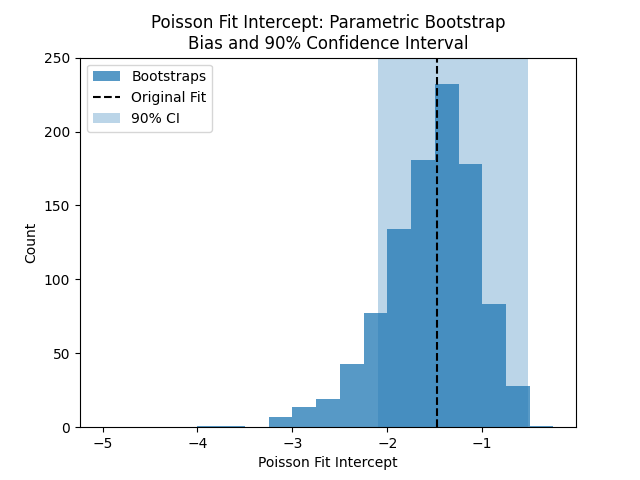
\includegraphics[width=4in,height=\textheight,keepaspectratio]{./images/fig3.png}

}

\subcaption{\label{fig-2b}Fit Intercepts}

\end{minipage}%

\caption{\label{fig-2}Histogram of Parametric Bootstrapped Poisson Fit
a. coefficients and b. intercepts, with the coefficient from the fit in
Figure~\ref{fig-1} shown dashed in black. 90\% Confidence inteval
highlighted in the background.}

\end{figure}%

For the coefficient, the bias is -0.0008, and the 90\% Basic Bootstrap
CI is (0.039, 0.215). For the intercept, the bias is 0.0721, and the
90\% Basic Bootstrap CI is (-0.522, -2.075).

\subsubsection{1.3}\label{section-2}

Based on the above plots, there is relatively low uncertainty about the
influence of ground cover on the expected number of salamanders. The
90\% CI ranges are not very wide for either the intercept or the
coefficient. More importantly, the CI is entirely above 0, which means
that the influence of a 1\% increase in ground cover on the number of
salamanders is always positive. We can also verify that the data is
likely a representative sample, since both statistics fall well within
the bootstrap CI, and the bias is low for both.

\newpage

\section{Problem 2: Norfolk Tide Gauge \& the Structured
Bootstrap}\label{problem-2-norfolk-tide-gauge-the-structured-bootstrap}

\subsubsection{2.1}\label{section-3}

\begin{figure}[h]

\centering{

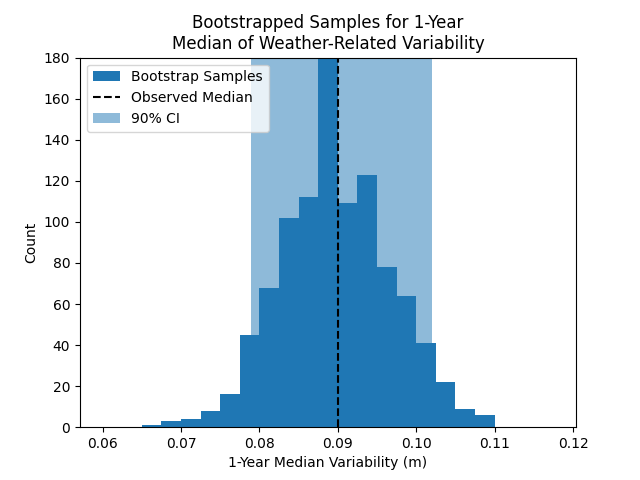
\includegraphics[width=5in,height=\textheight,keepaspectratio]{images/fig4.png}

}

\caption{\label{fig-4}Histogram of length-20 rolling block bootstrap
median weather-related tide variability, with the observed median shown
in black. The 90\% Confidence Interval is highlighted in the
background.}

\end{figure}%

The bias in the estimator is -0.00027, and the 90\% CI is (0.078,
0.103).

\newpage

\subsubsection{2.2}\label{section-4}

\begin{figure}[h]

\centering{

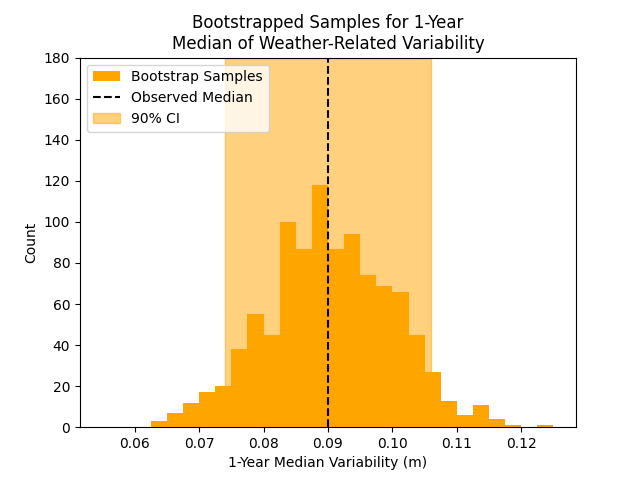
\includegraphics[width=5in,height=\textheight,keepaspectratio]{images/fig5.png}

}

\caption{\label{fig-5}Same as in Figure~\ref{fig-4}, but with length-50
block lengths.}

\end{figure}%

The bias in the estimator is 0.00083, and the 90\% CI is (0.073 0.106).
The bias is still very low/near-zero, although it did increase slightly.
The confidence interval widened, with the low-end decreasing by 0.003
and the high-end increasing by 0.005.

\subsubsection{2.3}\label{section-5}

Since the block sizes are larger, there are fewer blocks in each
bootstrapped time series, which makes the bootstrap sample medians more
susceptible to drawing a block with an outlier median. These extreme
blocks would have a larger effect on the bootstrap sample medians in a
length-50 bootstrap case than a length-20 case, thus explaining why the
CI expanded.

\newpage

\section{Problem 3: Chicago Deaths \& Missing
Data}\label{problem-3-chicago-deaths-missing-data}

\subsubsection{3.1}\label{section-6}

The \texttt{death}, \texttt{o3median}, \texttt{time}, and \texttt{tmpd}
columns have no missing data. For the others, there are:

\begin{itemize}
\tightlist
\item
  251 missing entries in \texttt{pm10median}
\item
  4387 missing entries in \texttt{pm25median}
\item
  27 missing entires in \texttt{so2median}
\end{itemize}

\subsubsection{3.2}\label{section-7}

\begin{figure}[H]

\begin{minipage}{0.50\linewidth}

\centering{

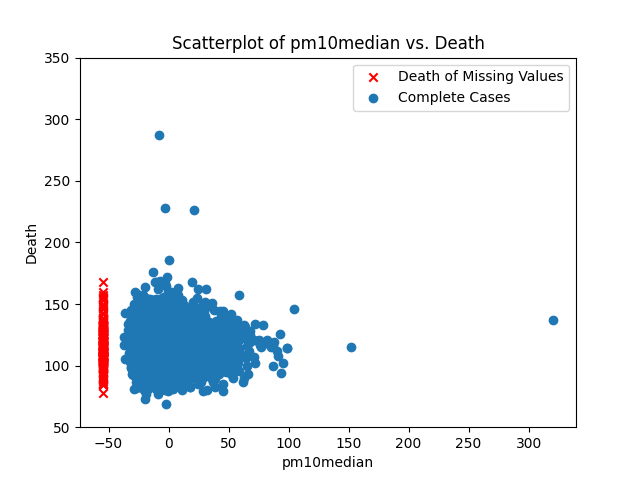
\includegraphics[width=4in,height=\textheight,keepaspectratio]{./images/fig6.png}

}

\subcaption{\label{fig-6a}Scatterplot of pm10median vs.~Death}

\end{minipage}%
%
\begin{minipage}{0.50\linewidth}

\centering{

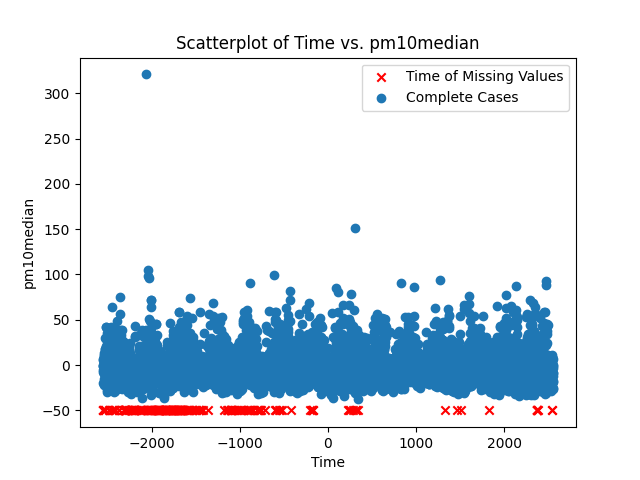
\includegraphics[width=4in,height=\textheight,keepaspectratio]{./images/fig7.png}

}

\subcaption{\label{fig-6b}Scatterplot of Time vs.~pm10median}

\end{minipage}%

\caption{\label{fig-6}Exploratory Data Analysis of missing values in the
chicago deaths dataset.}

\end{figure}%

In Figure~\ref{fig-6a}, the missing values for \texttt{pm10median}
appear to cover the distribution of \texttt{death} (with the exception
of the very high outliers), which suggests that the missingness is not
dependent on the y variable (\texttt{death} in this case, since we have
been focusing on predicting \texttt{death} with the environmental data).
However, in Figure~\ref{fig-6b}, the missing values seem to come
disproportionately from times earlier in the dataset. Since time is left
unmodeled when attempting to predict \texttt{death} from
\texttt{pm10median}, yet influences both, proceeding with complete-case
analysis will likely lead to skewed results due to this time dependence
of missing values. Thus, the \texttt{pm10median} data is Missing Not At
Random.




\end{document}
